\chapter{Results}
\label{sec:results}

This chapter reports the evaluation on the 150 test questions, answers each research
question in turn, and describes one change that was made during the evaluation. All
rates carry 95\% bootstrap intervals; differences are paired by question.

\section{Overview}

Figure~\ref{fig:outcomes} and Table~\ref{tab:main-results} summarise the five systems.
The full agent answered \nFullCorrect\% of the questions correctly, was wrong on
\nFullWrong\% and abstained on \nFullAbstain\%. Single-pass, which always answers, was
correct on \nSPCorrect\% and wrong on \nSPWrong\%. The text-only agent was correct on
\nTOCorrect\%, and the same full graph with Gemini behind it on \nGemCorrect\%.

\begin{figure}[htbp]
\centering
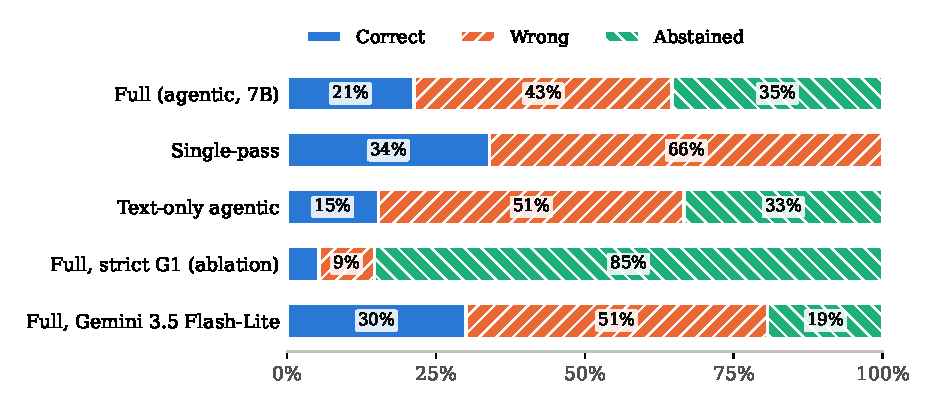
\includegraphics[width=\linewidth]{figures/fig_outcomes.pdf}
\caption{Outcomes on the 150 test questions. Correct and wrong as judged against
SPIQA's gold answer; abstained includes answers whose every claim was withheld.}
\label{fig:outcomes}
\end{figure}

% generated by scripts/make_thesis_tables.py -- do not edit
\begin{table}[htbp]
\centering
\scriptsize
\resizebox{\linewidth}{!}{%
\begin{tabular}{lccccccccc}
\toprule
System & Correct & Wrong & Abstained & Prec. & Hit & RF & AES & Search & Calls \\
\midrule
Full (agentic, 7B) & 21 [15, 28] & 43 [35, 51] & 35 [28, 43] & 33 & 0.73 & 0.44 & 0.44 & 2.7 & 11.7 \\
Single-pass & 34 [27, 41] & 66 [59, 73] & 0 [0, 0] & 34 & 0.77 & 0.41 & 0.36 & 3.0 & 3.0 \\
Text-only agentic & 15 [10, 21] & 51 [43, 59] & 33 [26, 41] & 23 & 0.00 & -- & 0.42 & 2.8 & 12.5 \\
Full, strict G1 (ablation) & 5 [2, 9] & 9 [5, 14] & 85 [79, 91] & 36 & 0.73 & 0.44 & 0.44 & 2.7 & 8.3 \\
Full, Gemini 3.5 Flash-Lite & 30 [23, 37] & 51 [43, 59] & 19 [13, 26] & 37 & 0.65 & 0.55 & 0.70 & 1.9 & 7.9 \\
\bottomrule
\end{tabular}}
\par\smallskip\parbox{0.95\linewidth}{\footnotesize Prec.\ = correct / answered (\%). Hit = the reference table or figure was retrieved. RF is undefined for text-only (it retrieves no region). Search = search-tool calls per question; Calls = model calls per question.}
\caption{Outcomes on the 150 test questions (\%, with 95\% bootstrap intervals), precision when answering, retrieval and efficiency. Correct and wrong are judged against SPIQA's gold answer by the model judge (Section~\ref{sec:judge}); abstained includes answers whose every claim was withheld by G2.}
\label{tab:main-results}
\end{table}


\paragraph{The judge.} The model judge agreed with the human grader on \nJudgeAgree{}
answers (Cohen's kappa~\cite{cohen1960kappa} \nJudgeKappa, substantial agreement); the
grader marked \nJudgeUnsure{} further answers as undecidable. In all three
disagreements the human called the answer correct and the judge wrong; the judge
never accepted an answer the human rejected. On the development questions, against
earlier hand labels, it agreed on 28 of 34 answers (kappa 0.64), and all six
disagreements concerned answers that were only partly right. The judge is therefore
reliable and, if anything, strict: the correct rates reported here are conservative
for every system, and all wrong rates are high partly because an incomplete answer
counts as wrong.

\section{RQ1: Does the Agentic Loop Improve Accuracy and Reduce Hallucination?}

\textbf{Answer: with the 7B model, the loop and its gates reduce wrong answers
substantially, but they do not raise accuracy: they trade correct answers for
abstentions, and the abstentions are not selective.}

The full agent is wrong \nDiffWrongSP{} percentage points less often than single-pass,
beyond luck (Table~\ref{tab:comparisons}). It is also correct \nDiffCorrectSP{} points
less often, again beyond luck, because it abstains on \nFullAbstain\% of the questions
where single-pass answers every one. Its precision when answering is no higher
(\nFullPrec\% against \nSPPrec\%): the reduction in wrong answers comes from answering
less, not from answering better.

% generated by scripts/make_thesis_tables.py -- do not edit
\begin{table}[htbp]
\centering
\small
\resizebox{\linewidth}{!}{%
\begin{tabular}{lccc}
\toprule
Comparison & Correct & Wrong & Abstained \\
\midrule
Full $-$ Single-pass (all 150) & -12.7 [-22, -4]$^{*}$ & -22.7 [-33, -13]$^{*}$ & +35.3 [+28, +43]$^{*}$ \\
Full $-$ Text-only (all 150) & +6.0 [-2, +14] & -8.0 [-18, +2] & +2.0 [-7, +12] \\
Full $-$ strict ablation (all 150) & +16.0 [+11, +22]$^{*}$ & +34.0 [+27, +41]$^{*}$ & -50.0 [-58, -42]$^{*}$ \\
Gemini $-$ Full (7B) (all 150) & +8.7 [+0, +17] & +7.3 [-2, +17] & -16.0 [-25, -7]$^{*}$ \\
Full $-$ Single-pass (multi-hop 10) & +20.0 [+0, +50] & -40.0 [-70, -10]$^{*}$ & +20.0 [+0, +50] \\
Full $-$ Text-only (multi-hop 10) & +40.0 [+10, +70]$^{*}$ & +0.0 [-30, +30] & -40.0 [-70, -10]$^{*}$ \\
Full $-$ strict ablation (multi-hop 10) & +60.0 [+30, +90]$^{*}$ & +20.0 [+0, +50] & -80.0 [-100, -50]$^{*}$ \\
Gemini $-$ Full (7B) (multi-hop 10) & -20.0 [-60, +20] & +10.0 [-30, +50] & +10.0 [-30, +50] \\
\bottomrule
\end{tabular}}
\caption{Paired differences in percentage points on the same questions, with 95\% bootstrap intervals (10{,}000 resamples). $^{*}$: the interval excludes 0.}
\label{tab:comparisons}
\end{table}


Table~\ref{tab:selectivity} makes this precise. A selective system would hold back the
questions that are hard for every system; single-pass's accuracy on those questions
would then be low. For the full agent it is the opposite: single-pass was correct on
\nSelFullHeld\% of the questions the agent held back, and on only \nSelFullAns\% of those
it answered. With the 7B model, the Sufficiency Gate's doubt does not track how hard a
question is. The best-effort flag tells the same story: answers given after the gate
stayed unconvinced were correct about as often as those it accepted (24 of 75 against
8 of 22).

% generated by scripts/make_thesis_tables.py -- do not edit
\begin{table}[htbp]
\centering
\small

\begin{tabular}{lcc}
\toprule
System & Held back & Answered \\
\midrule
Full (agentic, 7B) & 40 (of 53) & 31 (of 97) \\
Full, strict G1 (ablation) & 36 (of 128) & 23 (of 22) \\
Full, Gemini 3.5 Flash-Lite & 14 (of 29) & 39 (of 121) \\
\bottomrule
\end{tabular}
\caption{Is abstention selective? Single-pass's accuracy (\%) on the questions each system held back, and on those it answered. A selective system holds back the questions that are hard for every system.}
\label{tab:selectivity}
\end{table}


On the \nMultihopN{} multi-hop questions, where the plan expected the loop to matter most,
the picture is more favourable (Table~\ref{tab:multihop}): the agent was correct on 6
and wrong on 2, against 4 and 6 for single-pass; the difference in wrong answers is
beyond luck. With ten questions this is indicative only.

% generated by scripts/make_thesis_tables.py -- do not edit
\begin{table}[htbp]
\centering
\small

\begin{tabular}{lccc}
\toprule
System & Correct & Wrong & Abstained \\
\midrule
Full (agentic, 7B) & 6 & 2 & 2 \\
Single-pass & 4 & 6 & 0 \\
Text-only agentic & 2 & 2 & 6 \\
Full, strict G1 (ablation) & 0 & 0 & 10 \\
Full, Gemini 3.5 Flash-Lite & 4 & 3 & 3 \\
\bottomrule
\end{tabular}
\caption{Outcomes on the multi-hop subset (10 test questions that ask for a reason or an implication of a result: the result is in a table, the reason in the text). Counts.}
\label{tab:multihop}
\end{table}


The agent is also more economical in the sense of the planned efficiency score: it
calls the search tools 2.7 times per question against 3 for single-pass (AES 0.44
against 0.36, beyond luck). It is not cheaper overall: the planner and the gates cost
11.7 model calls per question against 3, and 27 seconds against 11 (medians).

\section{A Change Made During the Evaluation}
\label{sec:best-effort}

The design first frozen for the test run abstained whenever the Sufficiency Gate was
not convinced after three rounds. The first test run with it abstained on 110 of the
first 142 questions before a power cut stopped it --- although the reference table or
figure was in the buffer for about two thirds of them: the gate demanded that the
evidence state the answer outright, and the 7B model rarely saw it that way.

The plan's rule for a severe problem found during the test run was followed: fix it on
the development split only, re-freeze, re-run every system on the test split, and
report both runs. The change separates two decisions that the gate had merged. The
Sufficiency Gate decides when to \emph{stop searching}; whether a claim may be
\emph{published} is the Faithfulness Gate's job. After the last round, if the
Sufficiency Gate found facts that answer the question, the agent answers from them as
a flagged best effort, and every claim is still checked. On the development
questions this moved the full agent from 6 right, 1 partly right, 0 wrong and 13
abstentions to 9, 4, 5 and 2. A second idea, running every tool in the first round as
single-pass does, was tried on development and dropped: more evidence produced worse
conclusions (7, 5, 6, 2).

No test answer was read while making this change. The strict first design was kept
as an ablation and completed on all 150 questions: it abstained on \nStrictAbstain\%,
and of its 22 answers, 8 were correct and 14 wrong.

\section{RQ2: Can Visual Retrieval Fetch the Right Tables and Figures?}

\textbf{Answer: yes --- the reference table or figure reached the evidence buffer for
73\% of the questions --- but with the 7B model, being able to see tables and figures
changed accuracy little, except on multi-hop questions.}

Locating the reference works: the agent's buffer held it for 73\% of the questions,
single-pass's for 77\% (single-pass fetches every kind of evidence every time; the
agent chooses one per round). On development, ColQwen2 alone ranked the reference's
page first for 15 of 20 questions. Of the distinct tables and figures the agent
fetched, 44\% were the reference (RF), and 44\% of its published claims cite the
reference (the automatic stand-in for MAP, Table~\ref{tab:grounding}).

Against the text-only agent, which reads tables and figures only as extracted text,
the full agent was correct 6 points more often and wrong 8 points less often; neither
difference is beyond luck (Table~\ref{tab:comparisons}). On the multi-hop subset it was
correct 40 points more often, beyond luck. The two systems also abstain about equally
(\nFullAbstain\% and \nTOAbstain\%): the text-only agent's abstentions come from the same
gates.

\section{RQ3: Can the Agent Produce Precise Boxes?}
\label{sec:rq3}

\textbf{Answer: yes, when a claim cites the right table or figure: \nProofInsideFull\%
of such proof boxes land in the hand-drawn answer box, and every table-cell proof of
the full agent does (\nCellsFull). Per question, however, grounding scores are low,
because many questions are abstained and many proofs cite other sources.}

% generated by scripts/make_thesis_tables.py -- do not edit
\begin{table}[htbp]
\centering
\scriptsize
\resizebox{\linewidth}{!}{%
\begin{tabular}{lcccccc}
\toprule
System & CGS & CGS ans. & IoU$\geq$0.5 (\%) & Point. & Point. ans. & Ref.\ attr. \\
\midrule
Full (agentic, 7B) & 0.07 & 0.12 & 6 & 0.16 & 0.28 & 0.44 \\
Single-pass & 0.15 & 0.15 & 6 & 0.40 & 0.40 & 0.42 \\
Text-only agentic & 0.00 & 0.01 & 0 & 0.04 & 0.07 & 0.00 \\
Full, strict G1 (ablation) & 0.03 & 0.21 & 2 & 0.06 & 0.50 & 0.61 \\
Full, Gemini 3.5 Flash-Lite & 0.05 & 0.06 & 2 & 0.20 & 0.26 & 0.55 \\
\bottomrule
\end{tabular}}
\caption{Grounding on the 50 questions with hand-drawn answer boxes. CGS: best IoU of a proof box with a hand box (abstention = 0). Pointing: a proof box's centre lies inside a hand box. Ref.\ attr.: share of published claims citing the reference table or figure (all 150 questions).}
\label{tab:grounding}
\end{table}


Measured by IoU as planned, grounding is poor for every system: the full agent's CGS
is \nCGSFull{} (Table~\ref{tab:grounding}). Inspection showed that IoU penalises correct
proofs drawn at a different size from the hand box. On one question the agent boxed
exactly the two cells the gold answer names, but a parsed cell spans its whole column
(43~pt) while the hand box hugs the printed number (23~pt): IoU 0.43 and 0.46, below
the usual 0.5 threshold. A correct cell inside a hand box drawn around a whole row
scores 0.18. Shrinking every cited cell's box to its printed words did not help
(full 0.070 to 0.068): as many questions lost as gained. The pointing game, which asks
only whether a proof's centre lies inside a hand box, credits the full agent on
\nPointFullAns{} of its answered questions.

% generated by scripts/make_thesis_tables.py -- do not edit
\begin{table}[htbp]
\centering
\small
\resizebox{\linewidth}{!}{%
\begin{tabular}{lcccc}
\toprule
System & Proof boxes & On the reference & Inside the answer box & Table cells inside \\
\midrule
Full (agentic, 7B) & 72 & 31 & 22 (71\%) & 12/12 \\
Single-pass & 181 & 85 & 53 (62\%) & 30/44 \\
Full, Gemini 3.5 Flash-Lite & 68 & 28 & 13 (46\%) & 6/6 \\
\bottomrule
\end{tabular}}
\caption{Where the proof boxes point, on the annotated questions: boxes on the reference table or figure, and how many of those have their centre inside the hand-drawn answer box.}
\label{tab:proof-sources}
\end{table}


Table~\ref{tab:proof-sources} locates the problem. Of the full agent's \nProofBoxesFull{}
proof boxes on the annotated questions, only \nProofOnRefFull{} sit on the reference table
or figure; the rest point at paragraphs of text or at other tables. Where a proof does
sit on the reference, it points at the answer \nProofInsideFull\% of the time, and its
table-cell proofs all do. Single-pass, whose claims no gate checks, puts \nCellsSP{} of
its cell proofs on the answer. The boxing itself is precise; what limits grounding is
upstream --- which source a claim cites, and whether the question is answered at all.

\section{A Stronger Model Behind the Same Graph}

With Gemini~3.5 Flash-Lite behind every model call and nothing else changed, the
agent was correct on \nGemCorrect\%, wrong on \nGemWrong\% and abstained on \nGemAbstain\%;
its precision when answering was \nGemPrec\%. Its gates behaved differently from the
7B model's: the Sufficiency Gate was convinced on 117 questions instead of 22, after
fewer rounds (1.9 against 2.7), and the Faithfulness Gate kept 88\% of the drafted
claims instead of 50\%. Above all, its abstention was selective
(Table~\ref{tab:selectivity}): single-pass was correct on only \nSelGemHeld\% of the
questions Gemini held back, against \nSelGemAns\% of those it answered. Its retrieval was
also more focused (RF 0.55, AES 0.70). The difference in correct answers against the
7B agent, +8.7 points, sits at the edge of the interval ([0, +17]).
